\begin{frame}
    \frametitle{Factoring, motivation}
\note{Filename: ccsd\_factoring01.tex}

\small
\begin{block}{Diagram (2.12)}
    \begin{equation*}
        \parbox{40mm}{\includegraphics[scale=0.5]{graphics/ccsd_hbar_13_12}}
        = \frac{1}{4}  \bra{mn}\op{v}\ket{ef} t_{ij}^{ef} t_{mn}^{ab}
    \end{equation*}
\end{block}
\begin{block}{Diagram (2.26)}
    \begin{equation*}
        \parbox{40mm}{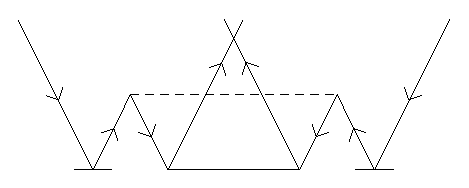
\includegraphics[scale=0.5]{graphics/ccsd_hbar_13_26}}
        = \frac{1}{4} P(ij) \bra{mn}\op{v}\ket{ef} t_i^e t_{mn}^{ab} t_j^f
    \end{equation*}
\end{block}
\begin{block}{Diagram (2.31)}
    \begin{equation*}
        \parbox{40mm}{\includegraphics[scale=0.5]{graphics/ccsd_hbar_13_31}}
        = \frac{1}{4} P(ij) P(ab) \bra{mn}\op{v}\ket{ef} t_i^e t_m^a t_j^f t_n^b
    \end{equation*}
\end{block}
\end{frame}

\begin{frame}
    \frametitle{Factoring, motivation}
\note{Filename: ccsd\_factoring02.tex}

\scriptsize
\begin{block}{Diagram (2.12)}
    \begin{equation*}
        \parbox{40mm}{\includegraphics[scale=0.5]{graphics/ccsd_hbar_13_12}}
        = \frac{1}{4}  \bra{mn}\op{v}\ket{ef} t_{ij}^{ef} t_{mn}^{ab}
    \end{equation*}
\end{block}
Diagram cost: $n_p^4 n_h^4$
\begin{block}{Diagram (2.12) - Factored}
\small
    \begin{align*}
        \parbox{40mm}{\includegraphics[scale=0.5]{graphics/ccsd_hbar_13_12}}
        &= \frac{1}{4}  \bra{mn}\op{v}\ket{ef} t_{ij}^{ef} t_{mn}^{ab} \\
        &= \frac{1}{4}  \left(\bra{mn}\op{v}\ket{ef} t_{ij}^{ef}\right)  t_{mn}^{ab} \\
        &= \frac{1}{4} X_{ij}^{mn} t_{mn}^{ab}
    \end{align*}
\end{block}
\end{frame}

\begin{frame}
    \frametitle{Factoring, motivation}
\note{Filename: ccsd\_factoring03.tex}

\small
\begin{block}{Diagram (2.26)}
    \begin{align*}
        \parbox{40mm}{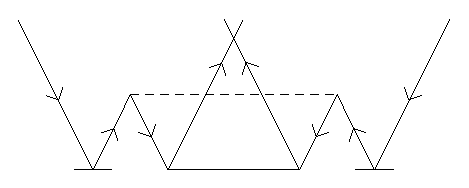
\includegraphics[scale=0.5]{graphics/ccsd_hbar_13_26}}
        &= \frac{1}{4} P(ij) \bra{mn}\ket{ef} t_i^e t_{mn}^{ab} t_j^f
    \end{align*}
\end{block}
Diagram cost: $n_p^4 n_h^4$
\begin{block}{Diagram (2.26) - Factored}
    \begin{align*}
        \parbox{40mm}{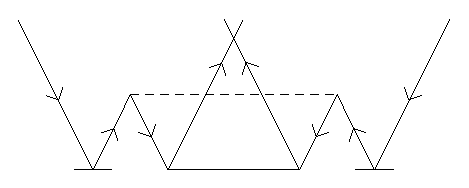
\includegraphics[scale=0.5]{graphics/ccsd_hbar_13_26}}
        &= \frac{1}{4} P(ij) \bra{mn}\op{v}\ket{ef} t_i^e t_{mn}^{ab} t_j^f \\
        &= \frac{1}{4} P(ij) t_{mn}^{ab} t_i^e X_{ej}^{mn} \\
        &= \frac{1}{4} P(ij) t_{mn}^{ab} Y^{mn}_{ij}
    \end{align*}
\end{block}
\end{frame}



\begin{frame}
    \frametitle{Factoring, motivation}
\note{Filename: ccsd\_factoring04.tex}

\scriptsize
\begin{block}{Diagram (2.31)}
    \begin{align*}
        \parbox{40mm}{\includegraphics[scale=0.5]{graphics/ccsd_hbar_13_31}}
        &= \frac{1}{4} P(ij) P(ab) \bra{mn}\op{v}\ket{ef} t_i^e t_m^a t_j^f t_n^b
    \end{align*}
\end{block}
Diagram cost: $n_p^4 n_h^4$
\begin{block}{Diagram (2.31) - Factored}
    \begin{align*}
        \parbox{40mm}{\includegraphics[scale=0.4]{graphics/ccsd_hbar_13_31}}
        &= \frac{1}{4} P(ij) P(ab) \bra{mn}\op{v}\ket{ef} t_i^e t_m^a t_j^f t_n^b \\
        &= \frac{1}{4} P(ij) P(ab) t_m^a t_n^b t_i^e X_{ej}^{mn} \\
        &= \frac{1}{4} P(ij) P(ab) t_m^a t_n^b Y_{ij}^{mn} \\
        &= \frac{1}{4} P(ij) P(ab) t_m^a Z_{ij}^{mb}
    \end{align*}
\end{block}
\end{frame}

\begin{frame}
    \frametitle{Factoring, Classification}
\note{Filename: ccsd\_factoring05.tex}

A diagram is classified by how many hole and particle lines between a $\hat{T}_i$ operator and the interaction ($T_i(p^{np} h^{nh})$).
\begin{block}{Diagram (2.12) Classification}
    \begin{equation*}
        \parbox{40mm}{\includegraphics[scale=0.5]{graphics/ccsd_hbar_13_12}}
        = \frac{1}{4}  \bra{mn}\op{v}\ket{ef} t_{ij}^{ef} t_{mn}^{ab}
    \end{equation*}
\end{block}
This diagram is classified as $T_2(p^2) \times T_2(h^2)$
\end{frame}

\begin{frame}
    \frametitle{Factoring, Classification}
\note{Filename: ccsd\_factoring06.tex}

\begin{block}{Diagram (2.26)} 
    \begin{equation*}
        \parbox{40mm}{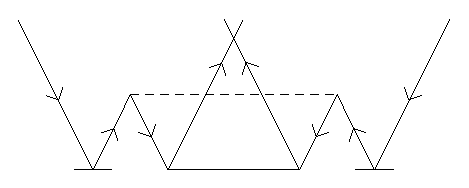
\includegraphics[scale=0.5]{graphics/ccsd_hbar_13_26}}
        = \frac{1}{4} P(ij) \bra{mn}\op{v}\ket{ef} t_i^e t_{mn}^{ab} t_j^f
    \end{equation*}
\end{block}
This diagram is classified as $T_2(h^2) \times T_1(p) \times T_1(p)$
\begin{block}{Diagram (2.31)} 
    \begin{equation*}
        \parbox{40mm}{\includegraphics[scale=0.5]{graphics/ccsd_hbar_13_31}}
        = \frac{1}{4} P(ij) P(ab) \bra{mn}\op{v}\ket{ef} t_i^e t_m^a t_j^f t_n^b
    \end{equation*}
\end{block}
This diagram is classified as $T_1(p) \times T_1(p) \times T_1(h) \times T_1(h)$
\end{frame}

